% status: 0
% chapter: TBD

\title{Analysis of Jaspersoft}


\author{Shagufta Pathan}
\orcid{1234-5678-9012}
\affiliation{%
  \institution{Indiana University}
  \streetaddress{}
  \city{Bloomington} 
  \state{IN} 
  \postcode{47408}
}
\email{spathan@iu.edu}

\author{Gregor von Laszewski}
\affiliation{%
  \institution{Indiana University}
  \streetaddress{Smith Research Center}
  \city{Bloomington} 
  \state{IN} 
  \postcode{47408}
  \country{USA}}
\email{laszewski@gmail.com}


% The default list of authors is too long for headers}
\renewcommand{\shortauthors}{G. v. Laszewski}


\begin{abstract}
Accessing information in today's world while the world competes on time and
information to gain competitive advantage, is still overly complex and
time-consuming for most business-people. Businesspeople need to access their
information, but typically do not have the time or inclination to do so in
specialized BI tools. This is where Jaspersoft comes into play. Jaspersoft
brings information to information workers, when and where they need it, by
embedding intelligence inside the application or portal, process or system that
they regularly use. This paper tries to introduce you to the Jaspersoft, its
architecture and some of its features and capabilities. 
\end{abstract}

\keywords{hid-sp18-516, Jaspersoft, reporting, analytics, BI}

\maketitle

\section{Introduction}
Jaspersoft is a Business Intelligence platform with reporting, analytics, data
visualization and data integration capabilities. It uses a commercial
open-source business model providing support for a variety of big data, mobile
and cloud deployments. It helps organizations in better decision-making with the
help of highly-interactive reports and
dashboards~\cite{hid-sp18-516-www-finances-online}. It allows its customers to
deliver efficiently by providing them with the self-serve capabilities to get
the answers they need inside their preferred apps or on their favorite
device~\cite{hid-sp18-516-www-jaspersoft-overview}. It scales architecturally
and economically to reach everyone to meet their business
goals~\cite{hid-sp18-516-www-finances-online}. 

Recently acquired by TIBCO in 2015~\cite{hid-sp18-516-www-wiki-jasperreports},
Jaspersoft is a BI software that is embedded in thousands of apps to reach
millions of information workers to enable better decision making each day. It
provides the ability to gain insight from various data sources and deliver
efficiently~\cite{hid-sp18-516-www-jaspersoft-overview}. Using an embedded BI
solution delivers state-of-the-art reporting and analytics saving the cost and
time of building one from scratch~\cite{hid-sp18-516-www-embedded-bi}. 


\section{Jaspersoft Community}
Jaspersoft provides two different editions: Jaspersoft BI Enterprise Edition and
Jaspersoft Studio Professional Edition. The Enterprise Edition is suitable for
Developers, BI administrators, business users and data analysts that lets them
build, deploy and manage reports, dashboards and data visualizations. The
Professional Edition is suitable for report developers, application developers
and BI experts. The Jaspersoft Studio Professional Edition is a desktop designer
used to build simple or complex reports and data visualizations, but don't need
the power of dashboards. The Professional Edition is basically used by
organizations who need business intelligence but do not need the same
capabilities as provided by the Enterprise
edition~\cite{hid-sp18-516-www-jaspersoft-download}.  


\section{Jaspersoft BI Solutions}
The Jaspersoft platform comprises of 3 main components: JasperReports Server,
Jaspersoft ETL and Jaspersoft Studio. Each of these components has a unique role
in powering the capabilities that Jaspersoft has to offer. The Jaspersoft
platform is built on Java and HTML5 within a flexible commercial open source
package. Let's look at each of these
platforms~\cite{hid-sp18-516-www-jaspersoft-quick-start}:

\subsection{JasperReports Server}
At the heart of Jaspersoft is the JasperReports Server. It is a stand-alone and
embeddable reporting server that provides reporting and analytics. It is used to
create dashboards and adhoc views and this is where all Jaspersoft content is
stored, accessed and distributed. It can be embedded into any mobile or web
application. It can also operate as a central information hub for the enterprise
to deliver mission critical information either in real-time or as per schedule
to the browser, mobile or email inbox in a variety of file formats. It builds on
JasperReports Library, which is a Java Library that offers an interface to the
JasperReports Library reporting
engine~\cite{hid-sp18-516-www-jasperreports-server}.
Figure~\ref{fig:jasperreports-server} shows the JasperReports Server
Architecture. The architecture includes data layer (it can take any data source
as input), configurable back-end layer, security layer, business layer providing
number of APIs, and user layer that includes the Web UI, Web Services and
Extensions to view and interact with the reports. All security is taken care by
Spring Framework~\cite{hid-sp18-516-www-jasperreports-server-architecture}. 

\begin{figure}[!ht]
	\centering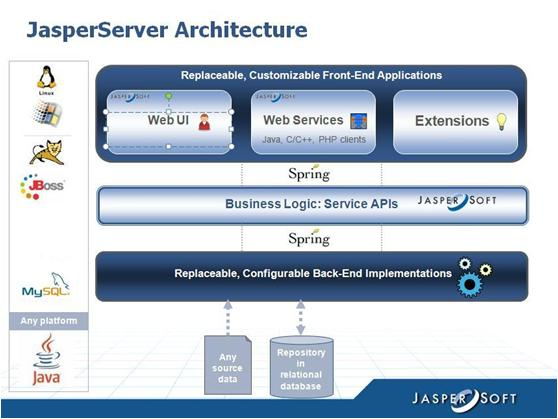
\includegraphics[width=\columnwidth]{../images/jasperreports-server.jpg}
	\caption{Architecture of JasperReports Server~\cite{hid-sp18-516-www-jasperreports-server-architecture}}
 	\label{fig:jasperreports-server}
\end{figure}

\subsection{Jaspersoft Studio}
The Jaspersoft Studio is a leading desktop tool for the creation of precision
reports with control over the finest details. It is the new Eclipse-based report
designer for JasperReports and JasperReports Server. It is available as
Eclipse~\cite{hid-sp18-516-www-eclipse} plugin, and as a standalone application.
Sophisticated layouts can be created which contain charts, images, subreports,
crosstabs and more can be created. Data can be accessed using different sources
through JDBC, TableModels, JavaBeans, XML, Hibernate, CSV, and custom sources,
and the reports can be published in a variety of formats as ``PDF, RTF, XML,
XLS, CSV, HTML, XHTML, text, DOCX, or
OpenOffice''~\cite{hid-sp18-516-www-jaspersoft-studio}. A report designed in
Jaspersoft Studio creates a JRXML file, which is an XML document that contains
the definition of the report layout. This layout is completely visual, and it
needs to be compiled before it can be executed. The compiled file is called
Jasper file which is a binary object. The report execution is done by passing
Jasper file and the data source to JasperReports, which is then able to generate
the final document in the format we want. Figures~\ref{fig:report-lifecycle}
and~\ref{fig:user-interface} shows the Report Lifecycle and the User Interface
as Eclipse plugin of the Jaspersoft studio
respectively~\cite{hid-sp18-516-www-jaspersoft-studio}.  

\begin{figure}[!ht]
        \centering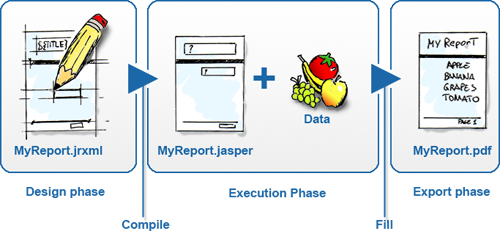
\includegraphics[width=\columnwidth]{../images/report-lifecycle.png}
        \caption{Report Lifecycle~\cite{hid-sp18-516-www-jaspersoft-studio}}
        \label{fig:report-lifecycle}
\end{figure}

\begin{figure}[!ht]
        \centering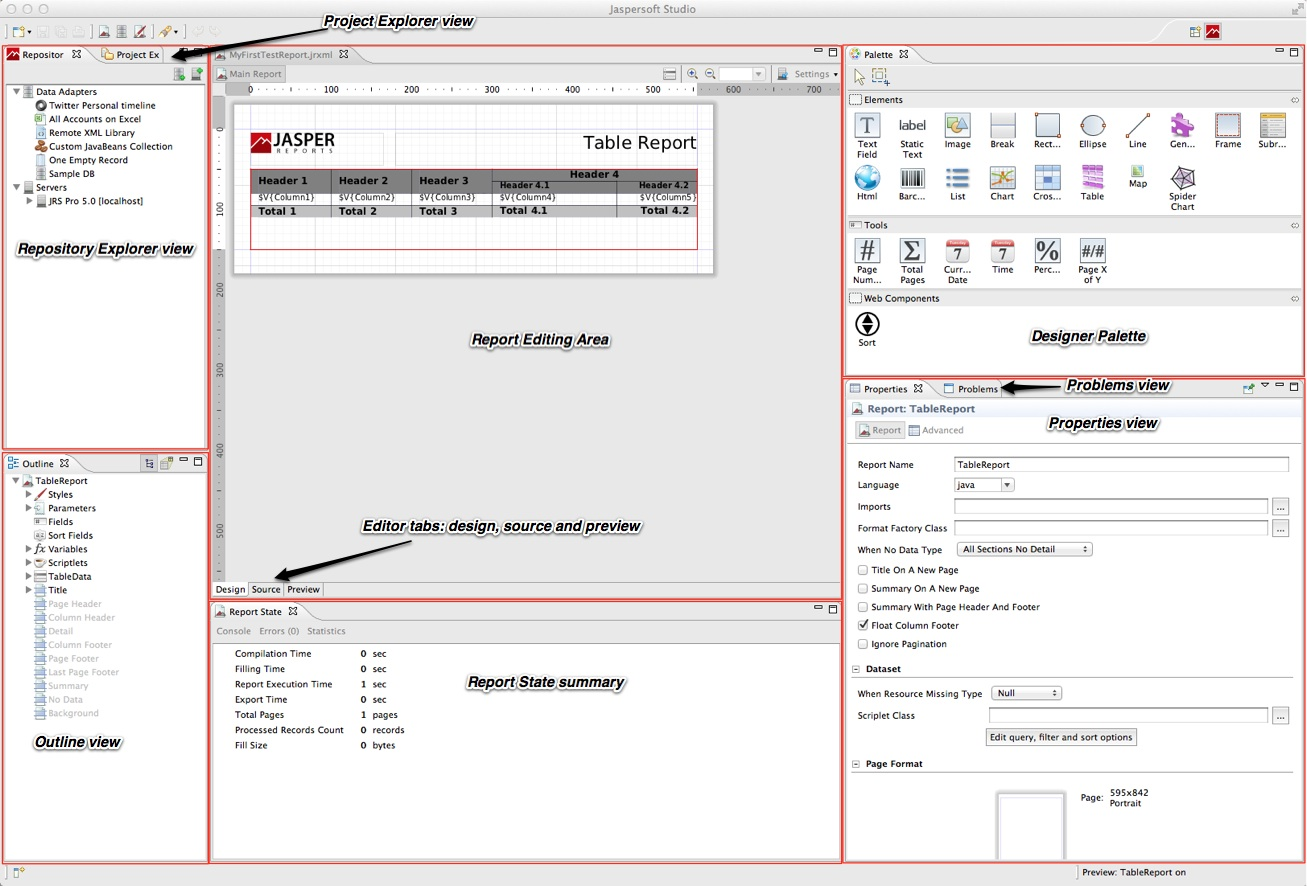
\includegraphics[width=\columnwidth]{../images/user-interface.jpg}
        \caption{User Interface~\cite{hid-sp18-516-www-jaspersoft-studio}}
        \label{fig:user-interface}
\end{figure}

\subsection{Jaspersoft ETL}
Finally, the Jaspersoft ETL bridges the divide between Jaspersoft and the data
sources by carefully tuning the ways in which the two interact. Jaspersoft's
comprehensive data integration software extracts and transforms data from
multiple systems and loads it into data stores optimized for reporting and
analysis data marts and warehouses. Several disparate relational or
non-relational data sources including files, web services, big data and
enterprise applications can be leveraged, combined and quickly connected. The
drag and drop process designer's predefined connectors and transformations can
be selected to create and test simple or sophisticated jobs that aggregate data
for visualizations, reporting and analysis requirements. With the ease of
built-in repository service, each job can be scheduled, reused or shared with
others. The integrated job monitoring dashboard gives instant insight into the
integration jobs with point-and-click access to ensure that the data management
is up-to-date and running smoothly at all times. Also due to the in-built
resiliency and scalability powered by its distributed architecture, it's easy to
synchronize volumes of data in real-time for more accurate decision
making~\cite{hid-sp18-516-www-data-integration}.


\section{Process}

The four key steps involved in distributing BI to its consumers across a
spectrum of channels that Jaspersoft applies which include~\cite{hid-sp18-516-www-quick-start-video}:
\begin{itemize} \item Platform: Choose a platform for Jaspersoft to be deployed onto.
\item Data: Data is fed in and organized. 
\item Author: The data fed is placed in the form of reports and dashboards.
\item Delivery: The reports and dashboards generated are then distributed
through a range of channels whether through email or as part of an
application~\cite{hid-sp18-516-www-quick-start-video}. \end{itemize}


\section{Capabilities/ Features}
Let's look at some of the main features of
Jaspersoft~\cite{hid-sp18-516-www-jaspersoft-features}:

\subsection{Reporting}
Jaspersoft's reporting software allows its customers to build any type of
reports including pixel-perfect for print layouts or interactive reports for web
and mobile applications. It can take information from one or more data sources
and produce information in an easy-to-read, highly interactive format for
business users. With its interactive report viewer, users can easily format,
filter, sort and restructure data to create their own personal report. This
interactively is automatically enabled which reduces the response time to user
interactions. The pixel-perfect reports are print-ready and can be published in
PDF, XLS, XML, DOC, JSON etc. Jaspersoft Studio, speeds development of
pixel-perfect and advanced reports. Jaspersoft also provides non-technical users
an easy-to-use drag-and-drop adhoc report designer, allowing them to build a
report on own their making it a self-service BI
tool~\cite{hid-sp18-516-www-jaspersoft-reporting-software}. 

\subsection{Analysis}
Jaspersoft's embeddable cost-effective reporting and data analytics software
allows users to quickly access, define and analyze any kind of data whether it's
in relational, Big Data or OLAP stores all through web-browser. Data can also be
accessed from NoSQL stores like MongoDB~\cite{hid-sp18-516-www-wiki-mongodb}
without requiring ETL. It's powerful analysis interface helps users to quickly
perform advanced data analysis in order to identify issues and spot trends. The
fast columnar in-memory engine allows to quickly explore data using interactive
html5 power charts and the multi-level zoom toolbar. It gives powers to end
users making their application more competitive to make better decisions
quickly~\cite{hid-sp18-516-www-jaspersoft-analytics-software}.

\subsection{Dashboard}
Jaspersoft's embedded dashboard solutions combines data and graphical indicators
to provide users with direct insight within their own applications. It gives
summaries of information for it users to view the state of their business and
quickly respond. Just like reporting, users can control data through external
filters with the help of embedded views. Along with gaining deeper insight into
application data, users can also enhance the look and feel of their application
with the help of these interactive dashboards. Users can also build and create
new reports or dashboards on their tablets with the fully featured mobile
dashboards. It provides server-side authentication for both mobile and tablet
devices to make decisions
securely~\cite{hid-sp18-516-www-jaspersoft-dashboards}. 

\subsection{Easy to integrate and maintain}
``Jaspersoft is based on modern REST web services, supports standard identity
management systems, provides built-in multi-tenancy support, and has a HTML5/CSS
driven user interface for easy re-branding. The result is a full featured set of
reporting and analytics capabilities made available in your Cloud-based or
locally deployed application, all in a matter of weeks, not 
months''~\cite{hid-sp18-516-www-embedded-bi}.


\section{Embedding Methods}
Jaspersoft's user interface can be embedded using three different methods:
Visualize.js, Iframes (HTTP APIs) and Web Services (REST APIs). Jaspersoft uses
Visualize.js to embed JasperReport Server reports and visualizations inside web
applications. It is a JavaScript API framework that is used to embed and
dynamically interact with reports. The look and feel of all the elements can be
controlled through CSS and new data can be merged into the application. Advanced
Business Intelligence can be made available to users with the help of
Visualize.js~\cite{hid-sp18-516-www-jaspersoft-visualize-js}. 

The HTTP Interface can be used to call Reports, Dashboards and parts of the
Jaspersoft application and is primarily used as shortcuts or entry points to
commonly used features or content. It can be embedded via
Iframes~\cite{hid-sp18-516-www-jaspersoft-http-api1}. The HTTP interface can't
be embedded in non-Jaspersoft applications, like the way web services and
Visualize.js APIs can be~\cite{hid-sp18-516-www-jaspersoft-http-api2}.

The components of JasperReports Server can be integrated into other applications
via the REST Web Service API calls by the hosting application. This includes
components repository services, scheduling services, Domain services and
administrative services. Authentication of the Web Service requests are done
using Spring Security and the web services can be configured to use
HTTPS~\cite{hid-sp18-516-www-jaspersoft-webservices}. 

\section{Platforms Supported}
Jaspersoft supports a variety of platforms to meet the needs of almost every
organization. It can be installed on different operating systems like Windows,
Linux, Unix and Apple macOS. It can be deployed in-premise, on cloud, in docker
containers~\cite{hid-sp18-516-www-docker} and also on Amazon Web Services 
(AWS)~\cite{hid-sp18-516-www-aws}. It supports different browsers including Firefox,
Internet Explorer and Edge, Apple Safari and Google Chrome. It supports different
types of data sources including relational, massively parallel databases like
Teradata~\cite{hid-sp18-516-www-techopedia-teradata}, Pivotal
Greenplum~\cite{hid-sp18-516-www-pivotal-greenplum}; many hosted databases like
Amazon Redshift~\cite{hid-sp18-516-www-aws-redshift}, Microsoft SQL
Azure~\cite{hid-sp18-516-www-microsoft-azure}, NoSQL Data sources like MongoDB,
Cassandra~\cite{hid-sp18-516-www-wiki-cassandra}, Big Data support for Hadoop
Hive~\cite{hid-sp18-516-www-wiki-hive},
Impala~\cite{hid-sp18-516-www-wiki-impala},
Spark~\cite{hid-sp18-516-www-wiki-spark} can be used. All Jaspersoft Editions
support application servers like Apache
Tomcat~\cite{hid-sp18-516-www-wiki-tomcat}~\cite{hid-sp18-516-www-jaspersoft-quick-start}.


\section{Jaspersoft and Big Data}
Jaspersoft gives the ability to work with Big Data by supporting native Big Data
functions for Native Connectors to connect and visualize data for Cassandra
Analytics, MongoDB Analytics, Hadoop Analytics and more. It provides users with
Real Time Analytics to connect and analyze data from these big data stores for
interactive reporting without having to move data through ETL. It also makes it
possible to blend data from relational databases with Big Data sources to
achieve a complete view of the business or customer for business users. This can
be achieved by blending data either through data virtualization metadata layer
or traditional data warehouse method using ETL.
Figures~\ref{fig:native-direct-access},~\ref{fig:blending-with-etl}
and~\ref{fig:blending-with-virtualization} shows the ways in which the data can
be blended~\cite{hid-sp18-516-www-jaspersoft-big-data}. 

\begin{figure}[!ht]
        \centering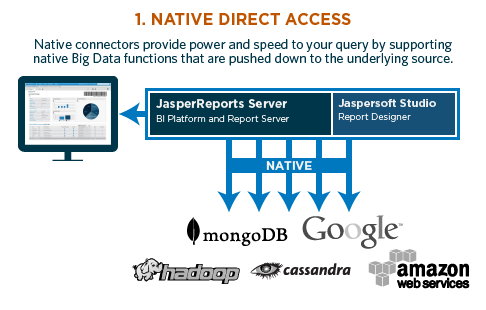
\includegraphics[width=\columnwidth]{../images/native-direct-access.png}
        \caption{Direct Access~\cite{hid-sp18-516-www-jaspersoft-big-data}}
        \label{fig:native-direct-access}
\end{figure}

\begin{figure}[!ht]
        \centering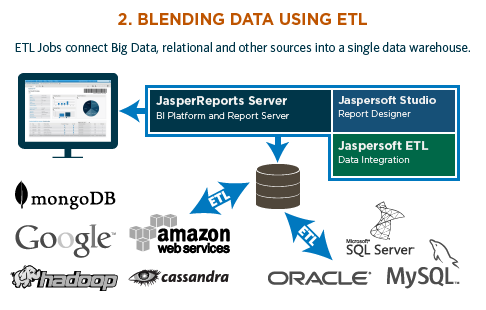
\includegraphics[width=\columnwidth]{../images/blending-with-etl.png}
        \caption{Blending Data with ETL~\cite{hid-sp18-516-www-jaspersoft-big-data}}
        \label{fig:blending-with-etl}
\end{figure}

\begin{figure}[!ht]
        \centering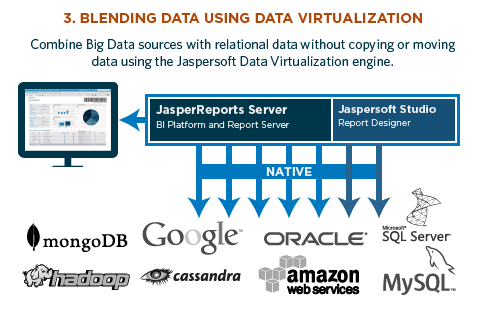
\includegraphics[width=\columnwidth]{../images/blending-with-virtualization.png}
        \caption{Blending Data with Virtualization~\cite{hid-sp18-516-www-jaspersoft-big-data}}
        \label{fig:blending-with-virtualization}
\end{figure}


\section{Licensing}
Jaspersoft Community Edition is licensed under the AGPL. The Enterprise and
Professional Edition is available to the users on a commercial license. It needs
to be purchased under a subscription model which offers different services and
support. Jaspersoft for AWS available on the AWS Marketplace provides the BI
software for less than \$1 per hour, paying only for what one
uses~\cite{hid-sp18-516-www-jaspersoft-licensing}. 


\section{Comparison with other BI Softwares}
Jaspersoft products compete with the other popular BI Softwares like
Pentaho~\cite{hid-sp18-516-www-pentaho},
Tableau~\cite{hid-sp18-516-www-tableau},
Sisense~\cite{hid-sp18-516-www-sisense}, and more. But Jaspersoft provides
features that are competitive enough compared to its equivalents. Jaspersoft has
got 100\% user satisfaction with respect to the other BI Softwares currently in
the market~\cite{hid-sp18-516-www-finances-online-comparisons}. 


\section{Conclusion}
Jaspersoft is a commercial open-source Business Intelligence platform embedded
with reporting, dashboards and data visualization capabilities. It is suitable
for small, medium and big business and provides data integration capabilities
for Big Data stores. It provides pixel-perfect documents with the use of data
from any data sources and brings timely, actionable data to users for faster
decision-making. It supports cloud and big data deployments and supports
multi-tenancy, multi-dimensional analytics by delivering data with usability,
security and integrity. 

\begin{acks}

  The authors would like to thank Dr.~Gregor~von~Laszewski for his
  support and suggestions to write this paper.

\end{acks}

\bibliographystyle{ACM-Reference-Format}
\bibliography{report} 

